\documentclass[twoside]{book}

% Packages required by doxygen
\usepackage{calc}
\usepackage{doxygen}
\usepackage{graphicx}
\usepackage[utf8]{inputenc}
\usepackage{makeidx}
\usepackage{multicol}
\usepackage{multirow}
\usepackage{textcomp}
\usepackage[table]{xcolor}

% Font selection
\usepackage[T1]{fontenc}
\usepackage{mathptmx}
\usepackage[scaled=.90]{helvet}
\usepackage{courier}
\usepackage{amssymb}
\usepackage{sectsty}
\renewcommand{\familydefault}{\sfdefault}
\allsectionsfont{%
  \fontseries{bc}\selectfont%
  \color{darkgray}%
}
\renewcommand{\DoxyLabelFont}{%
  \fontseries{bc}\selectfont%
  \color{darkgray}%
}

% Page & text layout
\usepackage{geometry}
\geometry{%
  a4paper,%
  top=2.5cm,%
  bottom=2.5cm,%
  left=2.5cm,%
  right=2.5cm%
}
\tolerance=750
\hfuzz=15pt
\hbadness=750
\setlength{\emergencystretch}{15pt}
\setlength{\parindent}{0cm}
\setlength{\parskip}{0.2cm}
\makeatletter
\renewcommand{\paragraph}{%
  \@startsection{paragraph}{4}{0ex}{-1.0ex}{1.0ex}{%
    \normalfont\normalsize\bfseries\SS@parafont%
  }%
}
\renewcommand{\subparagraph}{%
  \@startsection{subparagraph}{5}{0ex}{-1.0ex}{1.0ex}{%
    \normalfont\normalsize\bfseries\SS@subparafont%
  }%
}
\makeatother

% Headers & footers
\usepackage{fancyhdr}
\pagestyle{fancyplain}
\fancyhead[LE]{\fancyplain{}{\bfseries\thepage}}
\fancyhead[CE]{\fancyplain{}{}}
\fancyhead[RE]{\fancyplain{}{\bfseries\leftmark}}
\fancyhead[LO]{\fancyplain{}{\bfseries\rightmark}}
\fancyhead[CO]{\fancyplain{}{}}
\fancyhead[RO]{\fancyplain{}{\bfseries\thepage}}
\fancyfoot[LE]{\fancyplain{}{}}
\fancyfoot[CE]{\fancyplain{}{}}
\fancyfoot[RE]{\fancyplain{}{\bfseries\scriptsize Generated on Tue Apr 19 2016 12\-:49\-:34 for Actividad 2 by Doxygen }}
\fancyfoot[LO]{\fancyplain{}{\bfseries\scriptsize Generated on Tue Apr 19 2016 12\-:49\-:34 for Actividad 2 by Doxygen }}
\fancyfoot[CO]{\fancyplain{}{}}
\fancyfoot[RO]{\fancyplain{}{}}
\renewcommand{\footrulewidth}{0.4pt}
\renewcommand{\chaptermark}[1]{%
  \markboth{#1}{}%
}
\renewcommand{\sectionmark}[1]{%
  \markright{\thesection\ #1}%
}

% Indices & bibliography
\usepackage{natbib}
\usepackage[titles]{tocloft}
\setcounter{tocdepth}{3}
\setcounter{secnumdepth}{5}
\makeindex

% Hyperlinks (required, but should be loaded last)
\usepackage{ifpdf}
\ifpdf
  \usepackage[pdftex,pagebackref=true]{hyperref}
\else
  \usepackage[ps2pdf,pagebackref=true]{hyperref}
\fi
\hypersetup{%
  colorlinks=true,%
  linkcolor=blue,%
  citecolor=blue,%
  unicode%
}

% Custom commands
\newcommand{\clearemptydoublepage}{%
  \newpage{\pagestyle{empty}\cleardoublepage}%
}


%===== C O N T E N T S =====

\begin{document}

% Titlepage & ToC
\hypersetup{pageanchor=false}
\pagenumbering{roman}
\begin{titlepage}
\vspace*{7cm}
\begin{center}%
{\Large Actividad 2 }\\
\vspace*{1cm}
{\large Generated by Doxygen 1.8.6}\\
\vspace*{0.5cm}
{\small Tue Apr 19 2016 12:49:34}\\
\end{center}
\end{titlepage}
\clearemptydoublepage
\tableofcontents
\clearemptydoublepage
\pagenumbering{arabic}
\hypersetup{pageanchor=true}

%--- Begin generated contents ---
\chapter{Actividad 4}
\label{md_README}
\hypertarget{md_README}{}
Grupo C\-D\-I\-\_\-4

\begin{quotation}
Víctor Malvárez Filgueira

\end{quotation}


\begin{quotation}
Martín Molina Álvarez

\end{quotation}


\subsection*{Respuestas}

{\bfseries N\-O\-T\-A\-:} Los ejercicios marcados con un guión indican que no tienen una respuesta en forma de texto, sino que únicamente se entrega código.

\subsubsection*{1}


\begin{DoxyItemize}
\item \subsubsection*{2}
\end{DoxyItemize}


\begin{DoxyItemize}
\item \subsubsection*{3}
\end{DoxyItemize}


\begin{DoxyItemize}
\item \subsubsection*{4}
\end{DoxyItemize}

El método {\ttfamily notify\-All} notifica a todos los hilos que están esperando (han hecho {\ttfamily wait}) al objeto de dicho método. El método {\ttfamily notify} notifica únicamente a uno de los hilos que están esperando (no se sabe cuál, uno de ellos). En nuestro caso resulta conveniente utilizar el método {\ttfamily notify} ya que en cada instante solo un hilo va a estar a estar esperando que se despierte el propio objeto.

\subsubsection*{5}


\begin{DoxyItemize}
\item \subsubsection*{6}
\end{DoxyItemize}


\begin{DoxyItemize}
\item \subsubsection*{7}
\end{DoxyItemize}

?

\subsubsection*{8}




\begin{DoxyItemize}
\item El resultado debería ser constante ya que la pelota en cada momento solo puede estar en un jugador entonces es independiente del número de jugadores.
\item Las mediciones dicen que cuantos más hilos estén en funcionamiento (más jugadores) más lento es el programa.
\item El método más eficiente es con un número de jugadores entre 2-\/64 jugadores cuyos tiempos son muy similares (entre 35ms y 41ms).
\end{DoxyItemize}

\subsubsection*{9}

Si se interrupme un hilo el funcionamiento del programa no cambia. En cada jugador cuando se invoca el {\ttfamily wait()} se hace dentro de un bucle y un bloque {\ttfamily try catch} que comprueba si \char`\"{}sale del wait\char`\"{} de forma normal o por una interrupción. Para discernir si ha salido de forma normal utiliza como bandera la pelota. Si al salir del wait no tiene la pelota un bucle hace que vuelva a entrar en el wait. Código de ejemplo\-:

```java synchronized(this)\{ while(!tiene\-Pelota() \&\& !partida\-Finalizada)\{ this.\-esperando = true; try \{ this.\-wait(); \} catch(\-Interrupted\-Exception e)\{\}; this.\-esperando = false; \} \} ```

\subsubsection*{10}

Tuvimos que modificar este código\-:

```java

System.\-out.\-println(\char`\"{}\-El hilo \char`\"{} + id + \char`\"{} lanza la pelota\char`\"{});

\hyperlink{classActividad4_a23cf00e913eac32dea7597b617728047}{Actividad4.\-pasar\-Siguiente\-Jugador()};//pasa la pelota al siguiente jugador, en este caso a si mismo pelota=null;//se pasó la pelota a si mismo pero después la quitó entonces nunca sale del bucle por motivo de la expresión !tiene\-Pelota()

synchronized(this)\{ while(!tiene\-Pelota() \&\& !partida\-Finalizada)\{ this.\-esperando = true; try \{ this.\-wait(); \} catch(\-Interrupted\-Exception e)\{\}; this.\-esperando = false; \} \} ```

por este\-:

```java

System.\-out.\-println(\char`\"{}\-El hilo \char`\"{} + id + \char`\"{} lanza la pelota\char`\"{});

pelota=null; //\-A\-: quita la pelota antes de pasarla \hyperlink{classActividad4_a23cf00e913eac32dea7597b617728047}{Actividad4.\-pasar\-Siguiente\-Jugador()};//\-B\-: pasa la pelota al siguiente jugador, en este caso a si mismo

synchronized(this)\{ //no entra en el bucle por que en B\-: ha recibido la pelota (único jugador) while(!tiene\-Pelota() \&\& !partida\-Finalizada)\{ this.\-esperando = true; try \{ this.\-wait(); \} catch(\-Interrupted\-Exception e)\{\}; this.\-esperando = false; \} \} ``` 
\chapter{Hierarchical Index}
\section{Class Hierarchy}
This inheritance list is sorted roughly, but not completely, alphabetically\-:\begin{DoxyCompactList}
\item \contentsline{section}{Actividad4}{\pageref{classActividad4}}{}
\item \contentsline{section}{Pelota}{\pageref{classPelota}}{}
\item Runnable\begin{DoxyCompactList}
\item \contentsline{section}{Ping}{\pageref{classPing}}{}
\end{DoxyCompactList}
\end{DoxyCompactList}

\chapter{Class Index}
\section{Class List}
Here are the classes, structs, unions and interfaces with brief descriptions\-:\begin{DoxyCompactList}
\item\contentsline{section}{\hyperlink{classActividad4}{Actividad4} \\*Clase con todos los métodos estáticos que se encarga de iniciar y gestionar el juego }{\pageref{classActividad4}}{}
\item\contentsline{section}{\hyperlink{classPelota}{Pelota} }{\pageref{classPelota}}{}
\item\contentsline{section}{\hyperlink{classPing}{Ping} \\*Implementa los métodos relacionados con el jugador }{\pageref{classPing}}{}
\end{DoxyCompactList}

\chapter{File Index}
\section{File List}
Here is a list of all files with brief descriptions\-:\begin{DoxyCompactList}
\item\contentsline{section}{src/\hyperlink{Actividad4_8java}{Actividad4.\-java} }{\pageref{Actividad4_8java}}{}
\item\contentsline{section}{src/\hyperlink{Pelota_8java}{Pelota.\-java} }{\pageref{Pelota_8java}}{}
\item\contentsline{section}{src/\hyperlink{Ping_8java}{Ping.\-java} }{\pageref{Ping_8java}}{}
\end{DoxyCompactList}

\chapter{Class Documentation}
\hypertarget{classActividad4}{\section{Actividad4 Class Reference}
\label{classActividad4}\index{Actividad4@{Actividad4}}
}


Clase con todos los métodos estáticos que se encarga de iniciar y gestionar el juego.  


\subsection*{Static Public Member Functions}
\begin{DoxyCompactItemize}
\item 
static boolean \hyperlink{classActividad4_a646ea569d68870fe882316f81f57662b}{esta\-Partida\-Finalizada} ()
\item 
static void \hyperlink{classActividad4_a23cf00e913eac32dea7597b617728047}{pasar\-Siguiente\-Jugador} ()
\begin{DoxyCompactList}\small\item\em Pasa la pelota al siguiente jugador Pasa la pelota e incrementa el contador de jugadas. \end{DoxyCompactList}\item 
static void \hyperlink{classActividad4_a58b3e39e7248184ce102cf9c41cf393a}{main} (String\mbox{[}$\,$\mbox{]} args)
\begin{DoxyCompactList}\small\item\em Main. \end{DoxyCompactList}\end{DoxyCompactItemize}


\subsection{Detailed Description}
Clase con todos los métodos estáticos que se encarga de iniciar y gestionar el juego. 

\begin{DoxyAuthor}{Author}
marmol 
\end{DoxyAuthor}


\subsection{Member Function Documentation}
\hypertarget{classActividad4_a646ea569d68870fe882316f81f57662b}{\index{Actividad4@{Actividad4}!esta\-Partida\-Finalizada@{esta\-Partida\-Finalizada}}
\index{esta\-Partida\-Finalizada@{esta\-Partida\-Finalizada}!Actividad4@{Actividad4}}
\subsubsection[{esta\-Partida\-Finalizada}]{\setlength{\rightskip}{0pt plus 5cm}static boolean Actividad4.\-esta\-Partida\-Finalizada (
\begin{DoxyParamCaption}
{}
\end{DoxyParamCaption}
)\hspace{0.3cm}{\ttfamily [static]}}}\label{classActividad4_a646ea569d68870fe882316f81f57662b}
\hypertarget{classActividad4_a58b3e39e7248184ce102cf9c41cf393a}{\index{Actividad4@{Actividad4}!main@{main}}
\index{main@{main}!Actividad4@{Actividad4}}
\subsubsection[{main}]{\setlength{\rightskip}{0pt plus 5cm}static void Actividad4.\-main (
\begin{DoxyParamCaption}
\item[{String\mbox{[}$\,$\mbox{]}}]{args}
\end{DoxyParamCaption}
)\hspace{0.3cm}{\ttfamily [static]}}}\label{classActividad4_a58b3e39e7248184ce102cf9c41cf393a}


Main. 


\begin{DoxyParams}{Parameters}
{\em args} & Argumentos del programa \\
\hline
\end{DoxyParams}
\hypertarget{classActividad4_a23cf00e913eac32dea7597b617728047}{\index{Actividad4@{Actividad4}!pasar\-Siguiente\-Jugador@{pasar\-Siguiente\-Jugador}}
\index{pasar\-Siguiente\-Jugador@{pasar\-Siguiente\-Jugador}!Actividad4@{Actividad4}}
\subsubsection[{pasar\-Siguiente\-Jugador}]{\setlength{\rightskip}{0pt plus 5cm}static void Actividad4.\-pasar\-Siguiente\-Jugador (
\begin{DoxyParamCaption}
{}
\end{DoxyParamCaption}
)\hspace{0.3cm}{\ttfamily [static]}}}\label{classActividad4_a23cf00e913eac32dea7597b617728047}


Pasa la pelota al siguiente jugador Pasa la pelota e incrementa el contador de jugadas. 



The documentation for this class was generated from the following file\-:\begin{DoxyCompactItemize}
\item 
src/\hyperlink{Actividad4_8java}{Actividad4.\-java}\end{DoxyCompactItemize}

\hypertarget{classPelota}{\section{Pelota Class Reference}
\label{classPelota}\index{Pelota@{Pelota}}
}


The documentation for this class was generated from the following file\-:\begin{DoxyCompactItemize}
\item 
src/\hyperlink{Pelota_8java}{Pelota.\-java}\end{DoxyCompactItemize}

\hypertarget{classPing}{\section{Ping Class Reference}
\label{classPing}\index{Ping@{Ping}}
}


Implementa los métodos relacionados con el jugador.  


Inheritance diagram for Ping\-:\begin{figure}[H]
\begin{center}
\leavevmode
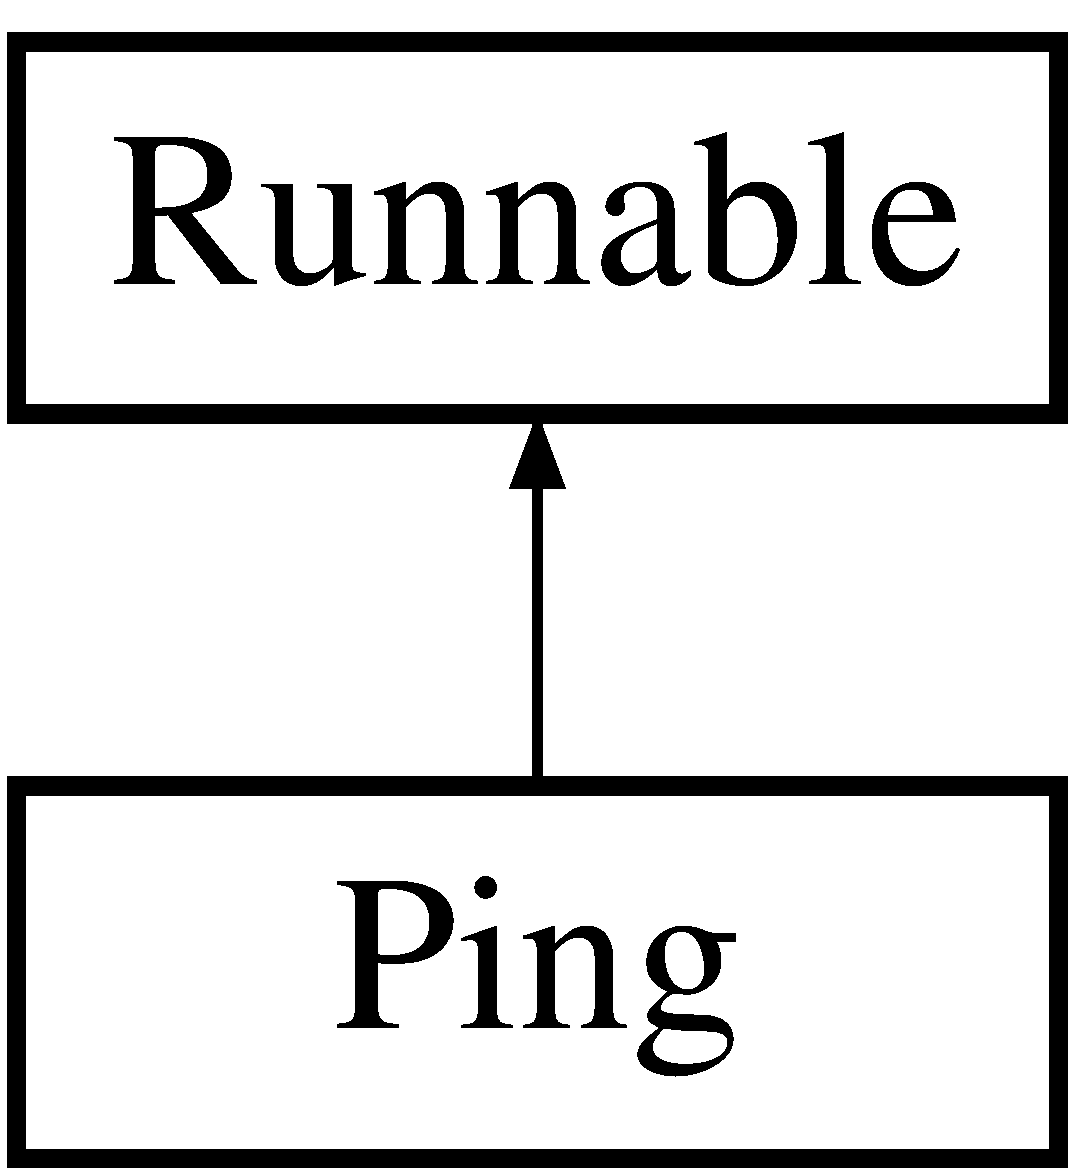
\includegraphics[height=2.000000cm]{classPing}
\end{center}
\end{figure}
\subsection*{Public Member Functions}
\begin{DoxyCompactItemize}
\item 
synchronized void \hyperlink{classPing_ade3b67ac253641d42d9a2057cfea7fe0}{recibir\-Pelota} (\hyperlink{classPelota}{Pelota} pelota)
\begin{DoxyCompactList}\small\item\em Recibe la pelota el jugador Este método nunca es invocado por el propio jugador. \end{DoxyCompactList}\item 
synchronized void \hyperlink{classPing_a6952252bb87045ab55691a79b53b5fe0}{finalizar\-Partida} ()
\begin{DoxyCompactList}\small\item\em Finaliza la partida. \end{DoxyCompactList}\item 
void \hyperlink{classPing_ad8528b6dfdff62253861d4881ecd2c43}{run} ()
\begin{DoxyCompactList}\small\item\em Método principal que invoca el thread. \end{DoxyCompactList}\end{DoxyCompactItemize}


\subsection{Detailed Description}
Implementa los métodos relacionados con el jugador. 

\begin{DoxyAuthor}{Author}
marmol 
\end{DoxyAuthor}


\subsection{Member Function Documentation}
\hypertarget{classPing_a6952252bb87045ab55691a79b53b5fe0}{\index{Ping@{Ping}!finalizar\-Partida@{finalizar\-Partida}}
\index{finalizar\-Partida@{finalizar\-Partida}!Ping@{Ping}}
\subsubsection[{finalizar\-Partida}]{\setlength{\rightskip}{0pt plus 5cm}synchronized void Ping.\-finalizar\-Partida (
\begin{DoxyParamCaption}
{}
\end{DoxyParamCaption}
)}}\label{classPing_a6952252bb87045ab55691a79b53b5fe0}


Finaliza la partida. 

\hypertarget{classPing_ade3b67ac253641d42d9a2057cfea7fe0}{\index{Ping@{Ping}!recibir\-Pelota@{recibir\-Pelota}}
\index{recibir\-Pelota@{recibir\-Pelota}!Ping@{Ping}}
\subsubsection[{recibir\-Pelota}]{\setlength{\rightskip}{0pt plus 5cm}synchronized void Ping.\-recibir\-Pelota (
\begin{DoxyParamCaption}
\item[{{\bf Pelota}}]{pelota}
\end{DoxyParamCaption}
)}}\label{classPing_ade3b67ac253641d42d9a2057cfea7fe0}


Recibe la pelota el jugador Este método nunca es invocado por el propio jugador. 


\begin{DoxyParams}{Parameters}
{\em pelota} & La pelota \\
\hline
\end{DoxyParams}
\hypertarget{classPing_ad8528b6dfdff62253861d4881ecd2c43}{\index{Ping@{Ping}!run@{run}}
\index{run@{run}!Ping@{Ping}}
\subsubsection[{run}]{\setlength{\rightskip}{0pt plus 5cm}void Ping.\-run (
\begin{DoxyParamCaption}
{}
\end{DoxyParamCaption}
)}}\label{classPing_ad8528b6dfdff62253861d4881ecd2c43}


Método principal que invoca el thread. 



The documentation for this class was generated from the following file\-:\begin{DoxyCompactItemize}
\item 
src/\hyperlink{Ping_8java}{Ping.\-java}\end{DoxyCompactItemize}

\chapter{File Documentation}
\hypertarget{README_8md}{\section{R\-E\-A\-D\-M\-E.\-md File Reference}
\label{README_8md}\index{R\-E\-A\-D\-M\-E.\-md@{R\-E\-A\-D\-M\-E.\-md}}
}

\hypertarget{Actividad4_8java}{\section{src/\-Actividad4.java File Reference}
\label{Actividad4_8java}\index{src/\-Actividad4.\-java@{src/\-Actividad4.\-java}}
}
\subsection*{Classes}
\begin{DoxyCompactItemize}
\item 
class \hyperlink{classActividad4}{Actividad4}
\begin{DoxyCompactList}\small\item\em Clase con todos los métodos estáticos que se encarga de iniciar y gestionar el juego. \end{DoxyCompactList}\end{DoxyCompactItemize}

\hypertarget{Pelota_8java}{\section{src/\-Pelota.java File Reference}
\label{Pelota_8java}\index{src/\-Pelota.\-java@{src/\-Pelota.\-java}}
}
\subsection*{Classes}
\begin{DoxyCompactItemize}
\item 
class \hyperlink{classPelota}{Pelota}
\end{DoxyCompactItemize}

\hypertarget{Ping_8java}{\section{src/\-Ping.java File Reference}
\label{Ping_8java}\index{src/\-Ping.\-java@{src/\-Ping.\-java}}
}
\subsection*{Classes}
\begin{DoxyCompactItemize}
\item 
class \hyperlink{classPing}{Ping}
\begin{DoxyCompactList}\small\item\em Implementa los métodos relacionados con el jugador. \end{DoxyCompactList}\end{DoxyCompactItemize}

%--- End generated contents ---

% Index
\newpage
\phantomsection
\addcontentsline{toc}{chapter}{Index}
\printindex

\end{document}
